\documentclass[10pt]{beamer}

\usetheme{metropolis}

\usepackage{booktabs}
\usepackage{array}
\usepackage[utf8]{inputenc}
\usepackage{pgfplots}
\usepackage{stmaryrd}
\usepackage{mathrsfs}
\usepackage{amsmath}
\usepackage{stmaryrd}
\usepackage{amsfonts}
\usepackage{movie15}
\usepackage{amssymb}
\usepackage{accsupp}
\usepackage{amsthm}
\usepackage{verbatim,cprotect}
\usepackage{listings}
\usepackage{hyperref}
\usepackage{enumerate}
\usepackage{tikz}
\usepackage[percent]{overpic}
\usepackage{tcolorbox}
\usepackage{color}
\usepackage{xspace}
\usepackage{alltt}
\usepackage{flushend}
\usepackage{graphicx}
\usepackage{wrapfig}
\usepackage[underline=false]{pgf-umlsd}

\usepackage[portuguese]{babel}
\usepackage[utf8]{inputenc}  % for proper diacritics
\usepackage[T1]{fontenc}
\usepackage {listings}
\usepackage{tikz}
% \usepackage{xcolor}
% Links
\usepackage{hyperref}

\usepackage{amsmath,amssymb}
%\usepackage{stmaryrd}
\usepackage{listings,color}
\usepackage{alltt}
\usepackage{flushend}



%\usepackage[T1]{fontenc}

% \lstdefinestyle{Go}{	
% 	keywordstyle=[1]\bfseries,
% 	basicstyle=\footnotesize\ttfamily,	
% 	numberstyle=\tiny,
% 	numbersep=5pt,
% 	breaklines=true,
% 	%prebreak=\raisebox{0ex}[0ex2][0ex]{\ensuremath{\hookleftarrow}},
% 	showstringspaces=false,
% 	upquote=true,
% 	tabsize=3,
% 	frame=tb,
% 	morekeywords={go,make,chan,int,import,main,func,for,select,case,string},
%       }

\lstdefinelanguage{Golang}%
  {morekeywords=[1]{package,import,func,type,struct,return,defer,panic,%
     recover,select,var,const,iota,},%
   morekeywords=[2]{string,uint,uint8,uint16,uint32,uint64,int,int8,int16,%
     int32,int64,bool,float32,float64,complex64,complex128,byte,rune,uintptr,%
     error,interface},%
   morekeywords=[3]{map,slice,make,new,nil,len,cap,copy,close,true,false,%
     delete,append,real,imag,complex,chan,},%
   morekeywords=[4]{for,break,continue,range,goto,switch,case,fallthrough,if,%
     else,default,},%
   morekeywords=[5]{Println,Printf,Error,Print,},%
   sensitive=true,%
   morecomment=[l]{//},%
   morecomment=[s]{/*}{*/},%
   morestring=[b]',%
   morestring=[b]",%
   morestring=[s]{`}{`},%
}

      
\lstdefinelanguage{SePi}%
  {morekeywords=[1]{type,integer,string,boolean,new, select, assume, assert},%
   sensitive=true,%
   morecomment=[l]{//},%
   morecomment=[s]{/*}{*/},%
   morestring=[b]',%
   morestring=[b]",%
   morestring=[s]{`}{`},%
 }

\lstdefinelanguage{CFST}%
{
  morekeywords=[1]{Int, Char, Bool, Skip, forall, rec, let, in, if, then, else, new, send, receive,
    select, fork, case, of, data, match, with},%  
  sensitive=true,%
  literate={->}{{$\rightarrow$}}1,%
   breaklines=true,
   morecomment=[l]{--},%
   morecomment=[s]{{-}{-}},%
   morestring=[b]',%
   morestring=[b]",%
   morestring=[s]{`}{`},%
 }

 

% notes
\newcommand{\todo}[1]{[{\color{blue}\textbf{#1}}]}

% Keywords
\newcommand{\keyword}[1]{\mathsf{#1}}

% Prekinds

\newcommand\prekind{\upsilon}

\newcommand{\stypes}{\mathcal S}
\newcommand\kinds{\stypes}

\newcommand{\types}{\mathcal T}
\newcommand\kindt{\types}

\newcommand\kindsch{\mathcal C}

% Multiplicity
\newcommand\Un{\ensuremath{\mathbf{u}}} % \infty
\newcommand\Lin{\ensuremath{\mathbf{l}}} % 1 

% Kinds
\newcommand\kind{\kappa}

% Grammars
\newcommand{\grmeq}{\; ::= \;}
\newcommand{\grmor}{\;\mid\;}

% type constructors
\newcommand\tcBase{B}
\newcommand\tcLolli\multimap
\newcommand\tcFun\to
\newcommand\tcBang{\mathop!}

% Keywords for types
\newcommand\kRec{\keyword{rec}}


% Types
\newcommand{\tskip}{\keyword{Skip}}
\newcommand\tSemi[2]{#1;#2}
\newcommand\tOut[1]{\tcBang#1}
\newcommand\tIn[1]{?#1}
\newcommand\tIChoice[1]{\oplus#1}
\newcommand\tEChoice[1]{\&#1}
\newcommand\tUnFun[2]{#1\tcFun#2}
\newcommand\tLinFun[2]{#1\tcLolli#2}
\newcommand\tPair[2]{#1\otimes#2}
\newcommand\tDatatype[1]{{[#1]}}
\newcommand\tRec[2]{\mu\,#1\,.\,#2}
\newcommand\tForall[2]{\forall\,#1\,.\,#2}

\newcommand\tRecK[2]{\kRec\,#1\,.\,#2}
% Environments
% \newcommand\emptyEnv{\cdot}
\newcommand\emptyEnv{\varepsilon}
\newcommand\kindEnv{\Delta}
\newcommand\varEnv{\Gamma}

% Language
% Expressions
% Language Types
\newcommand{\unite}{\keyword{Unit}}
\newcommand{\inte}{\keyword{Int}}
\newcommand{\chare}{\keyword{Char}}
\newcommand{\boole}{\keyword{Bool}}

% Variables
\newcommand\vare[1]{#1}
\newcommand\unlete[3]{\keyword{let} \; #1 = #2 \; \keyword{in} \; #3} 

% Applications
\newcommand\appe[2]{#1#2}
\newcommand\tappe[2]{#1[#2]}

% Conditional
\newcommand\conditionale[3]{\keyword{if}\;#1\;\keyword{then}\;#2\;\keyword{else} \; #3}

% Pairs
\newcommand\paire[2]{(#1,#2)}
\newcommand\binlete[4]{\keyword{let}\;#1, #2 = #3\;\keyword{in}\;#4}

% Session Types
\newcommand\newe[1]{\keyword{new}\;#1}
\newcommand\sende[2]{\keyword{send}\;#1\; #2}
\newcommand\recve[1]{\keyword{receive}\;#1}
\newcommand\selecte[1]{\keyword{select}\;#1}
\newcommand\matche[2]{\keyword{match}\;#1\;\keyword{with}\;#2}

% Fork
\newcommand\forke[1]{\keyword{fork}\;#1}

% Datatypes
\newcommand{\ctrcte}{C}
\newcommand\casee[2]{\keyword{case}\;#1\;\keyword{of}\;#2}

% Goal
\newcommand\Alg{\vdash_{a}}

% Equivalent
\newcommand\Equiv[2]{#1\,\thicksim\,#2}


%%% Local Variables:
%%% mode: latex
%%% TeX-master: "cfst-inforum18"
%%% End:
      
%\lstset{identifierstyle=\color{identifierColor}}

\title[FreeST]{\hfill 
\includegraphics[width=3cm]{img/normal} \\\vspace*{4mm} 
				\freest: Context-free session types in a functional language}

\date{
\vspace*{1cm}
\begin{center}
	April 2019
\end{center}}
\author[A.Mordido, V.Vasconcelos]{\underline{Bernardo Almeida}, Andreia Mordido, and Vasco T. Vasconcelos}
\institute[LASIGE, Faculdade de Ci\^encias, ULisboa]{LASIGE, Faculdade de Ci\^encias, Universidade de Lisboa \\\\
}
%\titlegraphic{\hfill
\includegraphics[height=1.5cm]{logo.png}}

\begin{document}
\lstset{language=freest, numbers=none}

\maketitle

\begin{frame}[fragile]{Motivation}
\vspace*{5mm}

\begin{lstlisting}
type TreeChannel = +{Leaf:Skip, 
                     Node:!Int;TreeChannel;TreeChannel}
\end{lstlisting}

\uncover<2->{
\begin{tabular}{lll}
	\freest\ & streams the tree on a \emph{single} channel\\
	& \emph{without} extraneous runtime checks.
\end{tabular}

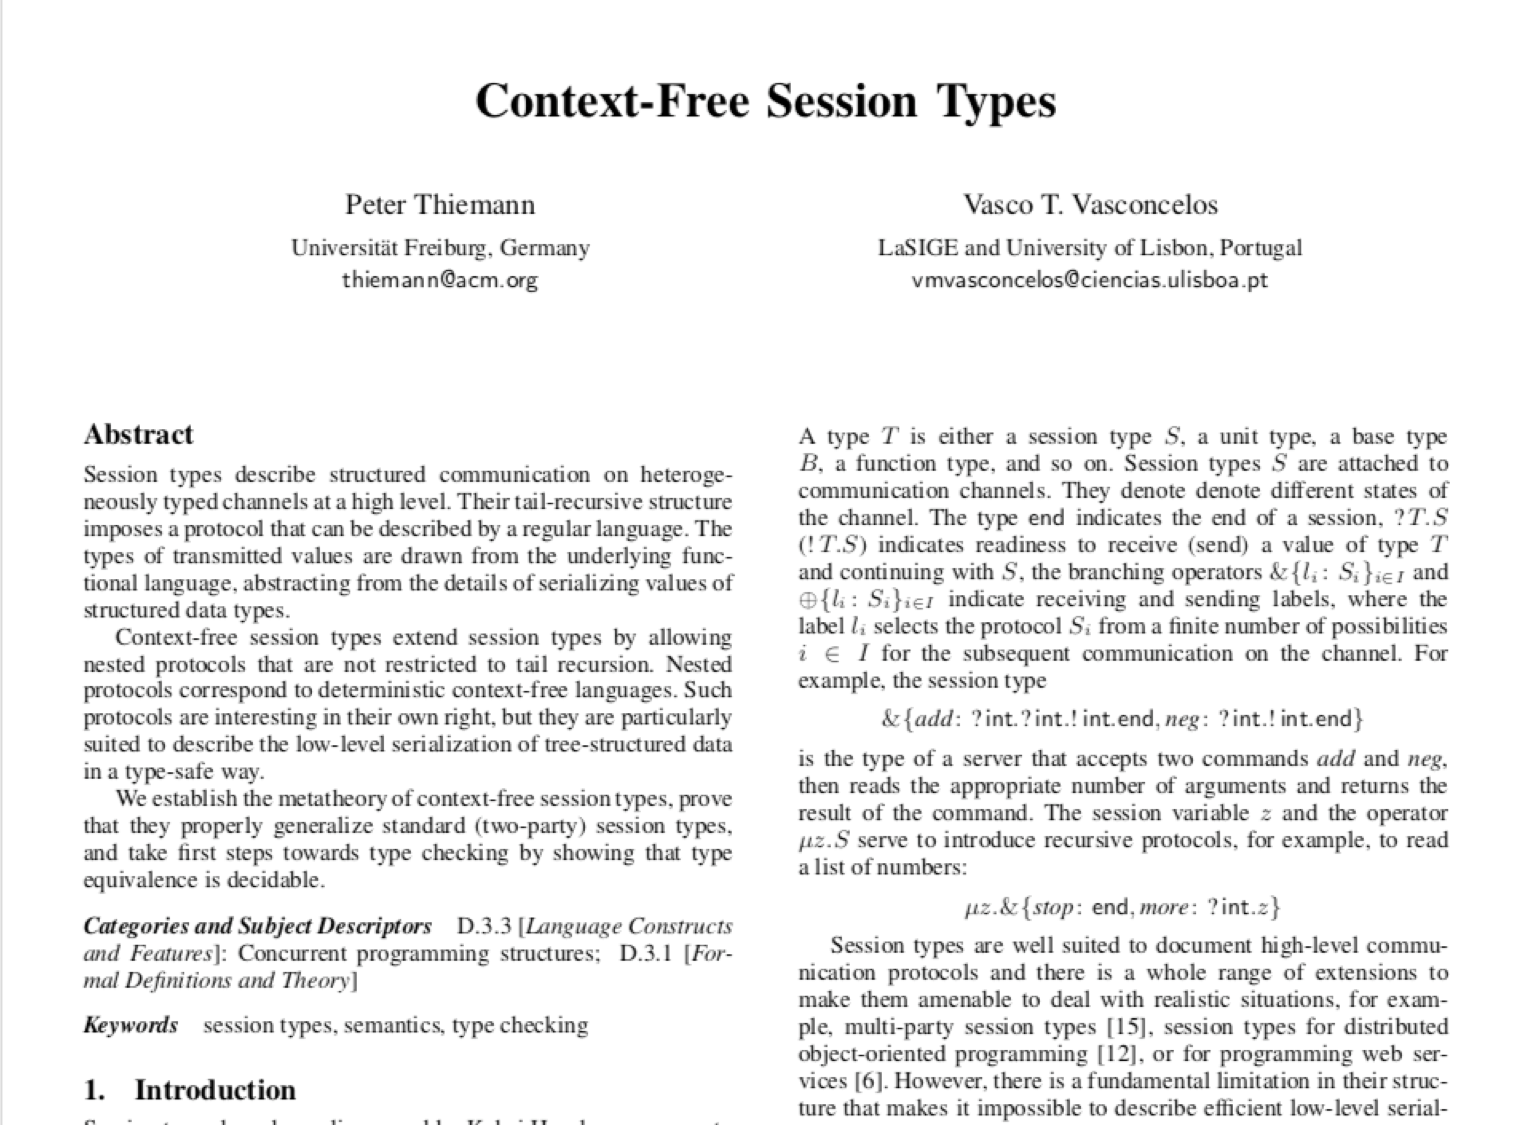
\includegraphics[width=7cm]{img/thiemann_vasconcelos.png}}
\hfill 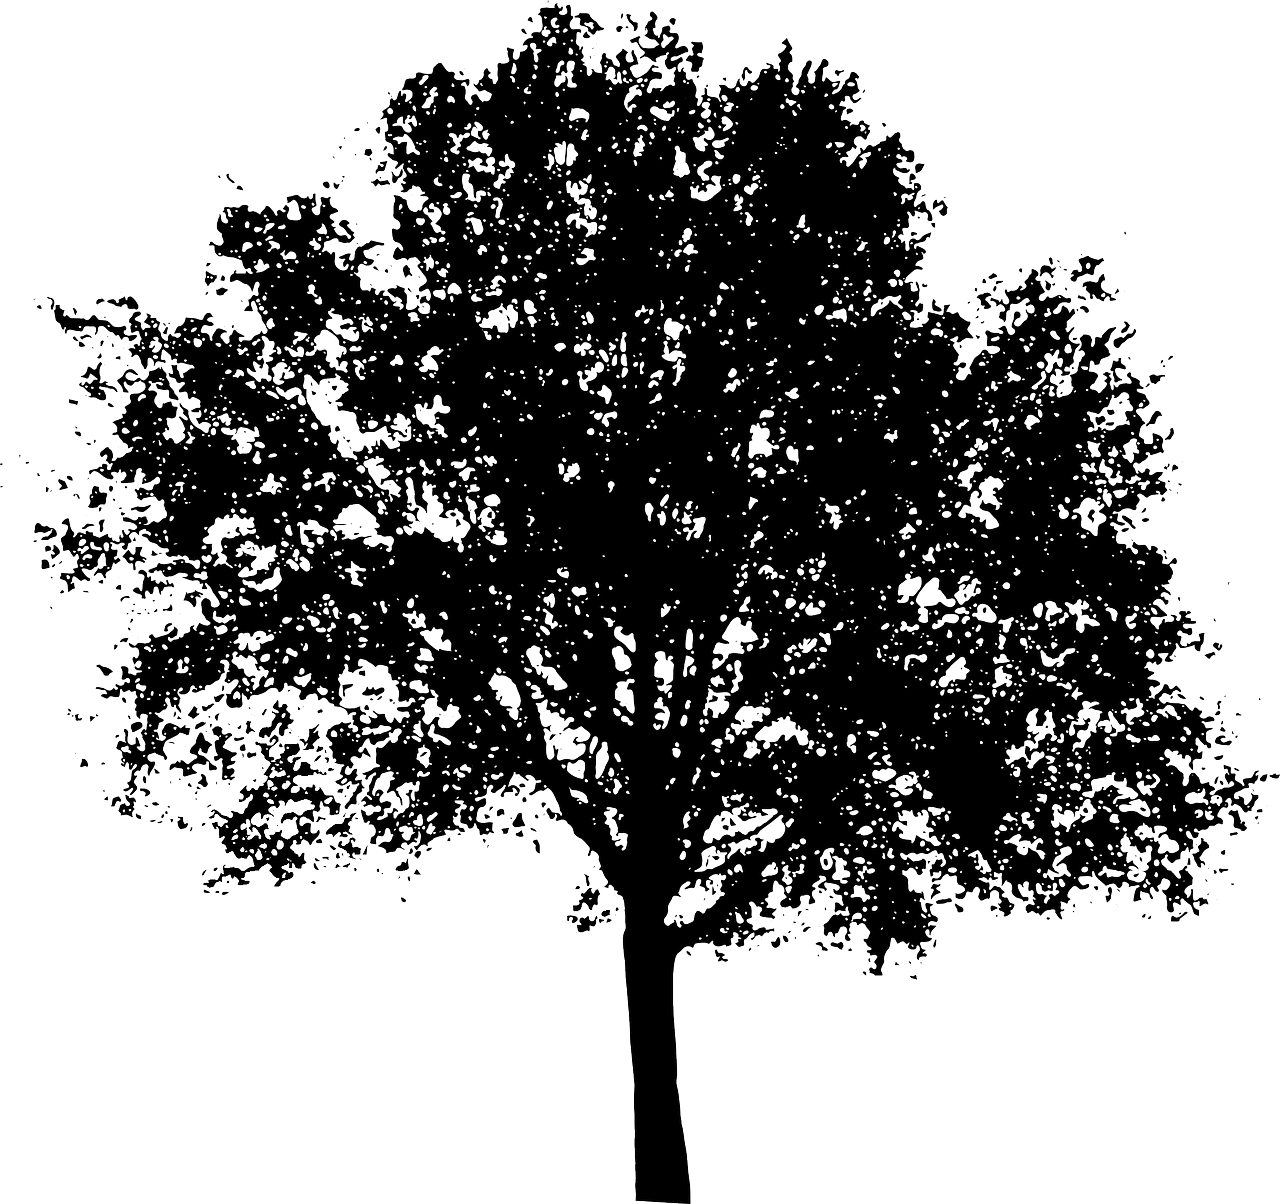
\includegraphics[height=3cm]{img/tree}
\end{frame}

%
\newcommand{\leaf}{$\bullet$}
%

\begin{frame}[fragile]{Example:  serialize a tree object on a channel \hfill \uncover<2->{\color{mLightBrown}writer}}
%\begin{center}
%  \begin{tikzpicture}[level 1/.style={sibling distance=2.2cm}, level
%    2/.style={sibling distance=1.5cm}, level 3/.style={sibling
%      distance=1.2cm}, level 4/.style={sibling distance=7mm}, level
%    distance = 7mm]
%    \node{\lstinline|1|} child { node {\lstinline|2|} child [level
%      3/.append style={sibling distance=7mm}]{ node {\lstinline|8|}
%        child { node {\leaf}} child { node {\leaf}}} child { node
%        {\lstinline|3|} child { node {\lstinline|5|} child { node
%            {\leaf}} child { node {\leaf}}} child { node
%          {\lstinline|4|} child { node {\leaf}} child { node {\leaf}}
%        }}} child[level 2/.append style={sibling distance=7mm}] { node
%      {\lstinline|6|} child { node {\leaf}} child[level 3/.append
%      style={sibling distance=7mm}] { node {\lstinline|7|} child {
%          node {\leaf}} child { node {\leaf}}}} ;
%  \end{tikzpicture}
%  \hspace*{2em}
%  \begin{tikzpicture}[level 1/.style={sibling distance=2.2cm}, level
%    2/.style={sibling distance=1.5cm}, level 3/.style={sibling
%      distance=1.2cm}, level 4/.style={sibling distance=7mm}, level
%    distance = 7mm]
%    \node{\lstinline|36|} child { node {\lstinline|22|} child [level
%      3/.append style={sibling distance=7mm}]{ node {\lstinline|8|}
%        child { node {\leaf}} child { node {\leaf}}} child { node
%        {\lstinline|12|} child { node {\lstinline|5|} child { node
%            {\leaf}} child { node {\leaf}}} child { node
%          {\lstinline|4|} child { node {\leaf}} child { node {\leaf}}
%        }}} child[level 2/.append style={sibling distance=7mm}] { node
%      {\lstinline|13|} child { node {\leaf}} child[level 3/.append
%      style={sibling distance=7mm}] { node {\lstinline|7|} child {
%          node {\leaf}} child { node {\leaf}}}} ;
%  \end{tikzpicture}
%\end{center}	

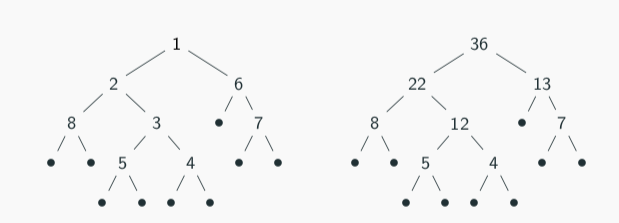
\includegraphics[width=11cm]{img/treesum}

\pause
\vspace{-4cm}
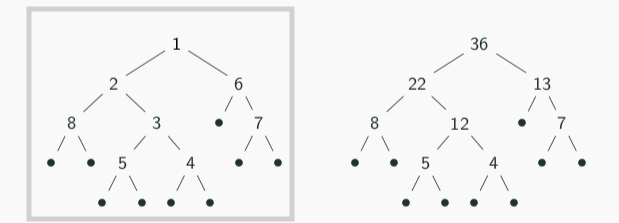
\includegraphics[width=11cm]{img/treesumL}
\pause

\begin{lstlisting}
type TreeC = +{Leaf: Skip, Node: !Int;TreeC;TreeC;?Int}
\end{lstlisting}
The type declaration introduces an \emph{abbreviation} to a recursive
type
\begin{lstlisting}
rec x. +{Leaf: Skip, Node: !Int;x;x;?Int}
\end{lstlisting}
that is \textbf{not} tail-recursive.
\end{frame}

\newcommand\hlmarkerstyle[5][yellow]{%
    \draw [ line width = \baselineskip, #1 ] (#2, #3) -- (#4, #5);
}
\let\hldefaultstyle=\hlmarkerstyle

\begin{frame}[fragile]{Example:  serialize a tree object on a channel \hfill{\color{mLightBrown}writer}}
	\textbf{Writer process}, writes a tree on a given channel:
	
\begin{lstlisting}
type TreeC = +{Leaf: Skip, Node: !Int;TreeC;TreeC;?Int}
\end{lstlisting}
\begin{lstlisting}[numbers=left, xleftmargin=0.7cm, escapeinside=\`\`]
transform: forall alpha => Tree -> TreeC;alpha -> (Tree, alpha)
transform tree c =
  case tree of
    Leaf ->
      (Leaf, select Leaf c)
    Node x l r ->
      let c  = select Node c in
      let c   = send x c in 
      let l,c = transform[TreeC;?Int;alpha] l c in
      let r,c = transform[?Int;alpha] r c in
      let y,c = receive c in
      (Node y l r, c)
\end{lstlisting}
\end{frame}

% select highlight
\begin{frame}[fragile]{Example:  serialize a tree object on a channel \hfill{\color{mLightBrown}writer}}
	\textbf{Writer process}, writes a tree on a given channel:
	
\begin{lstlisting}[escapeinside=\`\`]
type TreeC = +{Leaf: Skip,`\colorbox{yellow}{Node}`: !Int;TreeC;TreeC;?Int}
\end{lstlisting}
\begin{lstlisting}[numbers=left, xleftmargin=0.7cm, escapeinside=\`\`]
transform: forall alpha => Tree -> TreeC;alpha -> (Tree, alpha)
transform tree c =
  case tree of
    Leaf ->
      (Leaf, select Leaf c)
    Node x l r ->
      let c   = `\colorbox{yellow}{select}` Node c in
      let c   = send x c in 
      let l,c = transform[TreeC;?Int;alpha] l c in
      let r,c = transform[?Int;alpha] r c in
      let y,c = receive c in
      (Node y l r, c)
\end{lstlisting}
\end{frame}

% send highlight
\begin{frame}[fragile]{Example:  serialize a tree object on a channel \hfill{\color{mLightBrown}writer}}
	\textbf{Writer process}, writes a tree on a given channel:
	
\begin{lstlisting}[escapeinside=\`\`]
type TreeC = +{Leaf: Skip, Node: `\colorbox{yellow}{!Int}`;TreeC;TreeC;?Int}
\end{lstlisting}
\begin{lstlisting}[numbers=left, xleftmargin=0.7cm, escapeinside=\`\`]
transform: forall alpha => Tree -> TreeC;alpha -> (Tree, alpha)
transform tree c =
  case tree of
    Leaf ->
      (Leaf, select Leaf c)
    Node x l r ->
      let c   =  select Node c in
      let c   = `\colorbox{yellow}{send}` x c in 
      let l,c = transform[TreeC;?Int;alpha] l c in
      let r,c = transform[?Int;alpha] r c in
      let y,c = receive c in
      (Node y l r, c)
\end{lstlisting}
\end{frame}

% transform1 highlight
\begin{frame}[fragile]{Example:  serialize a tree object on a channel \hfill{\color{mLightBrown}writer}}
	\textbf{Writer process}, writes a tree on a given channel:
	
\begin{lstlisting}[escapeinside=\`\`]
type TreeC = +{Leaf: Skip, Node: !Int;`\colorbox{yellow}{TreeC}`;TreeC;?Int}
\end{lstlisting}
\begin{lstlisting}[numbers=left, xleftmargin=0.7cm, escapeinside=\`\`]
transform: forall alpha => Tree -> TreeC;alpha -> (Tree, alpha)
transform tree c =
  case tree of
    Leaf ->
      (Leaf, select Leaf c)
    Node x l r ->
      let c   = select Node c in
      let c   = send x c in 
      let l,c = `\colorbox{yellow}{transform}`[TreeC;?Int;alpha] l c in
      let r,c = transform[?Int;alpha] r c in
      let y,c = receive c in
      (Node y l r, c)
\end{lstlisting}
\end{frame}

% transform2 highlight
\begin{frame}[fragile]{Example:  serialize a tree object on a channel \hfill{\color{mLightBrown}writer}}
	\textbf{Writer process}, writes a tree on a given channel:
	
\begin{lstlisting}[escapeinside=\`\`]
type TreeC = +{Leaf: Skip, Node: !Int;TreeC;`\colorbox{yellow}{TreeC}`;?Int}
\end{lstlisting}
\begin{lstlisting}[numbers=left, xleftmargin=0.7cm, escapeinside=\`\`]
transform: forall alpha => Tree -> TreeC;alpha -> (Tree, alpha)
transform tree c =
  case tree of
    Leaf ->
      (Leaf, select Leaf c)
    Node x l r ->
      let c   = select Node c in
      let c   = send x c in 
      let l,c = transform [TreeC;?Int;alpha] l c in
      let r,c = `\colorbox{yellow}{transform}`[?Int;alpha] r c in
      let y,c = receive c in
      (Node y l r, c)
\end{lstlisting}
\end{frame}

% receive highlight
\begin{frame}[fragile]{Example:  serialize a tree object on a channel \hfill{\color{mLightBrown}writer}}
	\textbf{Writer process}, writes a tree on a given channel:
	
\begin{lstlisting}[escapeinside=\`\`]
type TreeC = +{Leaf: Skip, Node: !Int;TreeC;TreeC;`\colorbox{yellow}{?Int}`}
\end{lstlisting}
\begin{lstlisting}[numbers=left, xleftmargin=0.7cm, escapeinside=\`\`]
transform: forall alpha => Tree -> TreeC;alpha -> (Tree, alpha)
transform tree c =
  case tree of
    Leaf ->
      (Leaf, select Leaf c)
    Node x l r ->
      let c   = select Node c in
      let c   = send x c in 
      let l,c = transform [TreeC;?Int;alpha] l c in
      let r,c = transform[?Int;alpha] r c in
      let y,c = `\colorbox{yellow}{receive}` c in
      (Node y l r, c)
\end{lstlisting}
\end{frame}



\begin{frame}[fragile]{Example:  serialize a tree object on a channel\hfill{\color{mLightBrown}writer}}
	\textbf{Writer process}, writes a tree on a given channel:
	
\begin{lstlisting}
transform: forall alpha => Tree -> TreeC;alpha -> (Tree, alpha)
\end{lstlisting}
\begin{lstlisting}[numbers=left, xleftmargin=0.7cm, escapeinside=\`\`]
transform tree c =
  case tree of
    Leaf ->
      (Leaf, select Leaf c)
    Node x l r ->
      let `\colorbox{yellow}{c}`  = select Node c in
      let `\colorbox{yellow}{c}`   = send x c in 
      let l,`\colorbox{yellow}{c}` = transform[TreeC;?Int;alpha] l c in
      let r,`\colorbox{yellow}{c}` = transform[?Int;alpha] r c in
      let y,`\colorbox{yellow}{c}` = receive c in
      (Node y l r, c)
\end{lstlisting}

\end{frame}

\begin{frame}[fragile]{Example:  serialize a tree object on a channel\hfill{\color{mLightBrown}writer}}
	\textbf{Writer process}, writes a tree on a given channel:
	
\begin{lstlisting}[escapeinside=\`\`]
transform: forall `\colorbox{yellow}{$\alpha$}` => Tree -> TreeC;alpha -> (Tree, alpha)
\end{lstlisting}
\begin{lstlisting}[numbers=left, xleftmargin=0.7cm, escapeinside=\`\`]
transform tree c =
  case tree of
    Leaf ->
      (Leaf, select Leaf c)
    Node x l r ->
      let c  = select Node c in
      let c   = send x c in 
      let l,c = transform [`\colorbox{yellow}{TreeC;?Int;$\alpha$}`] l c in
      let r,c = transform [`\colorbox{yellow}{?Int;$\alpha$}`] r c in
      let y,c = receive c in
      (Node y l r, c)
\end{lstlisting}

\end{frame}

\begin{frame}[fragile]{Example:  serialize a tree object on a channel\hfill{\color{mLightBrown}reader}}

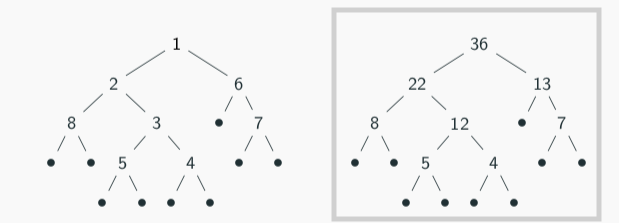
\includegraphics[width=11cm]{img/treesumR}
\pause

\begin{lstlisting}
type TreeS = &{Leaf: Skip, Node: ?Int;TreeS;TreeS;!Int}
\end{lstlisting}
Abbreviates the recursive type:
\begin{lstlisting}
rec x. &{Leaf: Skip, Node: ?Int;x;x;!Int}
\end{lstlisting}

\pause
\centering
\begin{tcolorbox}
	Type TreeC is \textbf{dual of} type TreeS.
\end{tcolorbox}

\end{frame}



\begin{frame}[fragile]{Example:  serialize a tree object on a channel\hfill{\color{mLightBrown}reader}}

\textbf{Reader process}, reads a tree on a given channel:
	
\begin{lstlisting}
treeSum: forall alpha => TreeS;alpha -> (Int, alpha)
\end{lstlisting}

\label{lst:treeSum}
\begin{lstlisting}[numbers=left,firstnumber=12, xleftmargin=0.7cm]
treeSum c =
  match c with
    Leaf c ->
      (0, c)
    Node c ->
      let x, c = receive c in
      let l, c = treeSum[TreeS;!Int;alpha] c in
      let r, c = treeSum[!Int;alpha] c in
      let c    = send (x + l + r) c in
      (x + l + r, c)
\end{lstlisting}
\end{frame}

\begin{frame}[fragile]{Example:  serialize a tree object on a channel\hfill{\color{mLightBrown}reader}}
	\textbf{Reader process}, reads a tree on a given channel:
	
\begin{lstlisting}
treeSum: forall alpha => TreeS;alpha -> (Int, alpha)
\end{lstlisting}

\label{lst:treeSum}
\begin{lstlisting}[numbers=left,firstnumber=12, xleftmargin=0.7cm, escapeinside=\`\`]
treeSum c =
  match c with
    Leaf c ->
      (0, c)
    Node c ->
      let x, `\colorbox{yellow}{c}` = receive c in
      let l, `\colorbox{yellow}{c}` = `\colorbox{yellow}{treeSum}`[TreeS;!Int;alpha] c in
      let r, `\colorbox{yellow}{c}` = `\colorbox{yellow}{treeSum}`[!Int;alpha] c in
      let `\colorbox{yellow}{c}`    = send (x + l + r) c in
      (x + l + r, c)
\end{lstlisting}

\end{frame}

\begin{frame}[fragile]{Example:  serialize a tree object on a channel}

Function \textbf{main} completes the program:

\begin{lstlisting}[escapeinside=\`\`]
treeSum: forall alpha => TreeS;alpha -> (Int, alpha)
transform: forall alpha => Tree -> TreeC;alpha -> (Tree, alpha)
\end{lstlisting}
\begin{lstlisting}[numbers=left,firstnumber=22, xleftmargin=0.7cm, escapeinside=\`\`]
main: Tree
main =
  let w,r = new TreeC in
  let _   = fork (treeSum[Skip] r) in
  let t,_ = transform[Skip] aTree w in
  t
\end{lstlisting}
\end{frame}


\begin{frame}[fragile]{Example:  serialize a tree object on a channel}

Function \textbf{main} completes the program:

\begin{lstlisting}[escapeinside=\`\`]
treeSum: forall `\colorbox{yellow}{$\alpha$}` => TreeS;alpha -> (Int, alpha)
transform: forall alpha => Tree -> TreeC;alpha -> (Tree, alpha)
\end{lstlisting}
\begin{lstlisting}[numbers=left,firstnumber=22, xleftmargin=0.7cm, escapeinside=\`\`]
main: Tree
main =
  let w,r = new TreeC in
  let _   = fork (treeSum[`\colorbox{yellow}{Skip}`] r) in
  let t,_ = transform[Skip] aTree w in
  t
\end{lstlisting}
\end{frame}

\begin{frame}[fragile]{Example:  serialize a tree object on a channel}

Function \textbf{main} completes the program:

\begin{lstlisting}[escapeinside=\`\`]
treeSum: forall alpha => TreeS;alpha -> (Int, `\colorbox{yellow}{$\alpha$}`)
transform: forall alpha => Tree -> TreeC;alpha -> (Tree, alpha)
\end{lstlisting}
\begin{lstlisting}[numbers=left,firstnumber=22, xleftmargin=0.7cm, escapeinside=\`\`]
main: Tree
main =
  let w,r = new TreeC in
  let `\colorbox{yellow}{$\_$}`  = fork (treeSum[Skip] r) in
  let t,_ = transform[Skip] aTree w in
  t
\end{lstlisting}
\end{frame}

\begin{frame}[fragile]{Example:  serialize a tree object on a channel}

Function \textbf{main} completes the program:

\begin{lstlisting}[escapeinside=\`\`]
treeSum: forall alpha => TreeS;alpha -> (Int, alpha)
transform: forall `\colorbox{yellow}{$\alpha$}` => Tree -> TreeC;alpha -> (Tree, alpha)
\end{lstlisting}
\begin{lstlisting}[numbers=left,firstnumber=22, xleftmargin=0.7cm, escapeinside=\`\`]
main: Tree
main =
  let w,r = new TreeC in
  let _   = fork (treeSum[Skip] r) in
  let t,_ = transform[`\colorbox{yellow}{Skip}`] aTree w in
  t
\end{lstlisting}
\end{frame}

\begin{frame}[fragile]{Example:  serialize a tree object on a channel}

Function \textbf{main} completes the program:

\begin{lstlisting}[escapeinside=\`\`]
treeSum: forall alpha => TreeS;alpha -> (Int, alpha)
transform: forall alpha => Tree -> TreeC;alpha -> (Tree, `\colorbox{yellow}{$\alpha$}`)
\end{lstlisting}
\begin{lstlisting}[numbers=left,firstnumber=22, xleftmargin=0.7cm, escapeinside=\`\`]
main: Tree
main =
  let w,r = new TreeC in
  let _   = fork (treeSum[Skip] r) in
  let t,`\colorbox{yellow}{$\_$} = transform[Skip] aTree w in
  t
\end{lstlisting}
\end{frame}

\begin{frame}[fragile]{Kinding}
	\freest\ requires kinding:
\begin{lstlisting}[escapeinside=\`\`]
!Int;?Bool `is a session type`
 Int->Bool `is a functional type`
\end{lstlisting}

\pause
\begin{tcolorbox}
\begin{lstlisting}[escapeinside=\`\`]
`\textbf{What about}` !Int;alpha `\textbf{?}`
\end{lstlisting}

\begin{lstlisting}[escapeinside=\`\`]
!Int;alpha `is a session type \textbf{only if}` alpha `is a session type`
\end{lstlisting}

\end{tcolorbox}		
\end{frame}

\begin{frame}{Kinding}
To accommodate polymorphism, types are classified into kinds:
$$ \textbf{Kind} = [\textbf{Prekind}][\textbf{Multiplicity}] $$

\textbf{Prekinds} distinguish:
\begin{itemize}
	\item functional types T
	\item session types S
\end{itemize}

\textbf{Multiplicities} control the number of times a value may be used in a context:
\begin{itemize}
	\item linear L, exactly one.
	\item unrestricted U, zero or more times
\end{itemize}

\pause
\vspace*{-1cm}

  \hspace*{7cm}\begin{tikzpicture}[scale=1]
    \node (TL) at (0,1) {\lstinline|TL|};
    \node (TU) at (-1,0) {\lstinline|TU|};
    \node (SL) at (1,0) {\lstinline|SL|};
    \node (SU) at (0,-1) {\lstinline|SU|};
    \draw (TL) -- (TU) -- (SU) -- (SL) -- (TL);
  \end{tikzpicture}

\vspace*{5mm}

\end{frame}

\begin{frame}{Kinding validates Types}
\freest{} features as functional types the following:
\begin{itemize}
\item \underline{Basic types}, \lstinline|B : TU|, that is, \lstinline|Int|,
  \lstinline|Bool|, \lstinline|Char|, and \lstinline|()|
\item \underline{Unrestricted and linear functions}, \lstinline|T1 -> T2 : TU| and
  \lstinline|T1 -o T2 : TL|
\item \underline{Pairs} \lstinline|(T1, T2)| of kind
  depending on the kinds of
  \lstinline|T1| and \lstinline|T2|, and
\item \underline{Datatypes}, \lstinline|[l1: T1, ..., ln: Tn]| of kind
  \lstinline|TU| or \lstinline|TL| depending on the kinds of the
  various types \lstinline|Ti|.
\end{itemize}
\pause

The session types are the following:
\begin{itemize}
\item \underline{Neutral}, \lstinline|Skip : SU|
\item \underline{Sequential composition}, \lstinline|S1;S2| of kind \lstinline|SU|
  or \lstinline|SL| depending on the kinds of \lstinline|S1| and
  \lstinline|S2|
\item  \underline{Messages}, \lstinline|!B, ?B|, both of kind \lstinline|SL|
\item \underline{Choices}, +\{l1: S1, ..., ln:Sn\}, \&\{l1: S1, ..., ln:Sn\},
  both of kind \lstinline|SL|
\item \underline{Recursive types}, \lstinline|rec x.S|, bearing the kind of
  \lstinline|S|.
\end{itemize}
	
\end{frame}

\begin{frame}[fragile]{One function, many forms}
	Polymorphic variables are introduced solely with the \lstinline|forall| construct.
	
	Function \lstinline|transform| introduces the kind for the
        polymorphic type variable~\lstinline|alpha|:
        
        \begin{center}
          \lstinline|forall alpha:SL => Tree -> TreeC;alpha -> (Tree,alpha)|
        \end{center}
\pause
\begin{lstlisting}[numbers=left, xleftmargin=0.7cm, escapeinside=\`\`, basicstyle=\sffamily\scriptsize]
transform tree c =
  case tree of
    Leaf ->
      (Leaf, select Leaf c)
    Node x l r ->
      let c   = select Node c in
      let c   = send x c in 
      let l,c = transform[`\colorbox{yellow!60}{TreeC;?Int;$\alpha$}`] l c in
      let r,c = transform[`\colorbox{yellow!60}{?Int;$\alpha$}`] r c in
      let y,c = receive c in
      (Node y l r, c)
\end{lstlisting}
\pause
In line 8, \lstinline|transform| calls the function at (monomorphic) type:
\begin{lstlisting}
Tree -> TreeC;TreeC;?Int;alpha -> (Tree, TreeC;?Int;alpha)
\end{lstlisting}
	
\end{frame}

\begin{frame}{Expressions {\small \color{mLightBrown}inspired in functional languages}}
\freest{} blends expressions typical of functional languages:
\begin{itemize}
\item \underline{Basic values}: \lstinline|Int|,
  \lstinline|Bool|, \lstinline|Char|, and \lstinline|()|
\item \underline{Term variables} (as opposed to type variables)
\item \underline{Lambda introduction}: 
\begin{itemize}
	\item \lstinline|\x -o e| for linear abstractions
	\item \lstinline|\x -> e| for unrestricted abstractions
\end{itemize}
\item \underline{Lambda elimination}, \lstinline|e1 e2|
\item \underline{Pair introduction}, \lstinline|(e1,e2)| 
\item \underline{Pair elimination},
  \lstinline|let x, y = e1 in e2| %(linear versions only)
\item \underline{Datatype elimination},
  \lstinline|case e of \{l1 x11...x1k -> e1; ...; ln xn1...xnk -> en\}|
\item \underline{Conditional}, \lstinline|if e1 then e2 else e3|
\item \underline{Type application}, \lstinline|x[T1,...Tn]|
\item \underline{Thread creation}, \lstinline|fork e|.
\end{itemize}
\end{frame}

\begin{frame}{Expressions {\small \color{mLightBrown}inspired in session types}}
The session-type related expressions are:
\begin{itemize}
\item \underline{Channel creation}, \lstinline|new S|
\item \underline{Messages} \lstinline|send e| and
  \lstinline|receive e|
\item \underline{Branch selection}, \lstinline|select l e|
\item \underline{Branch match},
  \lstinline|match e with \{l1 x -> e1;...;ln x -> en\}|.
\end{itemize}
\end{frame}

\begin{frame}{Programs}
Programs are composed by
%
\begin{itemize}
\item Function signatures and
  declarations
\item Datatype declarations
\item Type abbreviations.
\end{itemize}
\end{frame}

\begin{frame}{Type equivalence}
	The compiler embeds an algorithm to check type equivalence:
	\begin{center}
    	\begin{tikzpicture}[node distance = 2.5cm, auto]
      		% Place nodes
      		\node [block2] (typeToGrammar) {{\bf Convert types to a context-free grammar}\\ Translates types into a set of productions}; 
      		\node [block2,below=5mm of typeToGrammar] (prune) {{\bf Prune unnormed productions}\\ Streamlines the grammar by pruning unnormed productions};%
      		\node [block2,below=5mm of prune] (simplifyExpand) {{\bf Simplify and expand}\\ Alternates between simplification and expansion operations, until reaching a successful branch in the expansion tree or concluding that all branches are unsuccessful };
      		% Draw edges
      		\path [line] (typeToGrammar) -- (prune);
      		\path [line] (prune) -- (simplifyExpand);
   		\end{tikzpicture}
  	\end{center}
  	\begin{tcolorbox}
  		The algorithm to check type equivalence is sound and complete!
  	\end{tcolorbox}

\end{frame}

\begin{frame}[fragile]{Code generation}

\freest{} is written in Haskell and \textbf{generates Haskell code} that can be
compiled with a GHC compiler. \pause

%We build on modules \lstinline|Control.Concurrent| and \lstinline|Unsafe.Coerce|. % , and use:
\vskip 1cm
%\begin{tcolorbox}
The three possible runtimes:
\begin{itemize}
   \item Synchronous channels\pause
   \item Asynchronous channels\pause
   \item \lstinline|MVar|s                  
\end{itemize}	
%\end{tcolorbox}
% \begin{lstlisting}[language=Haskell]
% (>>) :: Monad m => m a -> m b -> m b
% (>>=) :: Monad m => m a -> (a -> m b) -> m b
% return :: Monad m => a -> m a
% \end{lstlisting}

% \pause
% To fork a new thread, we use the forkIO primitive:

% \begin{lstlisting}[language=Haskell]
% fork :: IO () -> IO ()
% fork e = forkIO e >> return ()
% \end{lstlisting}

\end{frame}

% \begin{frame}[fragile]{Code generation}
% \begin{tcolorbox}
% 	The three possible runtimes:
% 	\begin{itemize}
% 		\item Synchronous channels
% 		\item Asynchronous channels
% 		\item \lstinline|MVar|s                  
% 	\end{itemize}	
% \end{tcolorbox}
% \end{frame}

\begin{frame}[fragile]{Runtime}

Each channel is implemented with a pair of \lstinline|MVar|s:
\begin{lstlisting}
type ChannelEnd a b = (MVar a, MVar b)
\end{lstlisting}

\pause
The \lstinline|new| function creates such a pair and returns the two
channel ends in a pair:

\begin{lstlisting}[language=Haskell, literate={<-}{{$\leftarrow$}}1]
new :: IO (ChannelEnd a b, ChannelEnd b a)
new = do
  m1 <- newEmptyMVar
  m2 <- newEmptyMVar
  return ((m1, m2), (m2, m1))
\end{lstlisting}
\end{frame}

\begin{frame}[fragile]{Runtime \hfill {\color{mLightBrown} write on a channel end}}

\begin{tcolorbox}
\begin{itemize}
        \item We use the first MVar to read from a channel and the second one to write on that channel. \pause
%        \item We use the second \lstinline|MVar| to write on a channel. \pause
	\item We use unsafeCoerce to bypass the Haskell type system (only when reading and writing from \lstinline|MVar|s). \pause
	\item To write on the channel end we use the \lstinline|putMVar| primitive and \lstinline|takeMVar| to read.\pause
	%\item If the \lstinline|MVar| is full, \lstinline|putMVar| waits until it becomes empty. \pause
	\item The result of \lstinline|send| is the original channel end, which must be rebound in programs.
        \item The result of \lstinline|receive| is a pair composed of the value read from the \lstinline|MVar| and the original channel.

\end{itemize}
\end{tcolorbox}

\lstinline|MVar|s  implement \emph{asynchronous} channels with
buffers of size one. 

% \pause
% \begin{lstlisting}[language=Haskell, literate={<-}{{$\leftarrow$}}1]
% send :: b -> ChannelEnd a b -> IO (ChannelEnd a b)
% send x (m1, m2) = putMVar m2 (unsafeCoerce x) >> return (m1, m2)
% \end{lstlisting}

\end{frame}

%\begin{frame}[fragile]{Runtime \hfill {\color{mLightBrown} read from a channel end}}

% \begin{tcolorbox}
% \begin{itemize}
% 	\item We use the first MVar to read from a channel. \pause
% 	\item The \lstinline|takeMVar| primitive returns the contents of the
% \lstinline|MVar|. \pause
% 	\item If the \lstinline|MVar| is empty,
% \lstinline|takeMVar| waits until it is full. \pause
% 	\item After a
% \lstinline|takeMVar|, the \lstinline|MVar| is left empty.\pause
% \item The result
% of \lstinline|receive| is a pair composed of the value read from the
% \lstinline|MVar| and the original channel.
% \end{itemize}
% \end{tcolorbox}

% \pause
% \begin{lstlisting}[language=Haskell, literate={->}{{$\rightarrow$}}1]
% receive :: ChannelEnd a b -> IO (a, ChannelEnd a b)
% receive (m1, m2) = takeMVar m1 >>= \x -> return (unsafeCoerce x, (m1, m2))
% \end{lstlisting}

%\end{frame}

\begin{frame}[fragile]{Example}

In the following program
\lstinline|w1|-\lstinline|r1| and \lstinline|w2|-\lstinline|r2| are
two channels.
%
\begin{lstlisting}
writer :: !Char -> !Bool -> Skip
writer w1 w2 =
  let _ = send 'c' w1 in
  send False w2
reader :: ?Char -> ?Bool -> Bool
reader r1 r2 =
  let x, _ = receive r2 in
  let _, _ = receive r1 in
  x
\end{lstlisting}
%
The program deadlocks with synchronous channels but not with MVars or
asynchronous channels.	
\end{frame}

\begin{frame}[fragile]{The bright future of FreeST}
Possible extensions to the language:
\begin{itemize}
	\item Allow messages of arbitrary types, rather than basic
          types alone %\lstinline|!S| rather than only \lstinline|!B|.
	\item Incorporate type inference on type applications.
	\item Support for linear pairs, linear datatypes, and polymorphic datatypes.
%	\item Instead of a buffered semantics with a buffer of size 1, we plan to have buffered channels of arbitrary size.
	\item Play with call-by-need (rather than call-by-value) operational semantics.
\end{itemize}

% Already done:
% \begin{itemize}
% 	\item Incorporation of the \lstinline|dualof| type operator.
% \end{itemize}
	
\end{frame}

\plain{Thank you!}

{\setbeamercolor{background canvas}{bg=white}
\begin{frame}{Algorithmic kinding system}
	\hspace*{-8mm}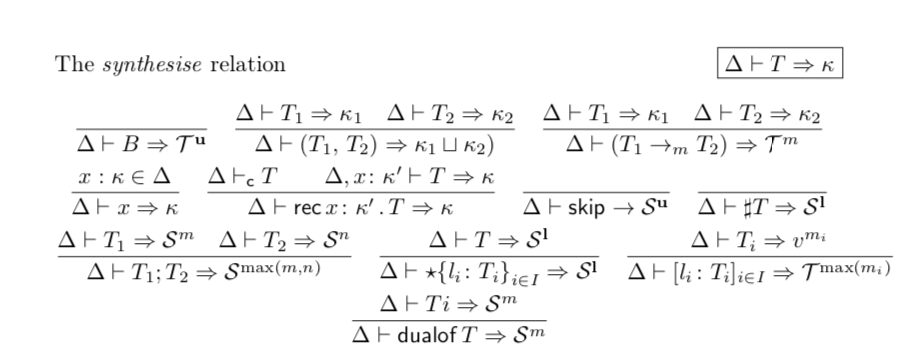
\includegraphics[width=12cm]{img/synthesise}
\end{frame}

\begin{frame}{Algorithmic kinding system}
	\hspace*{-8mm}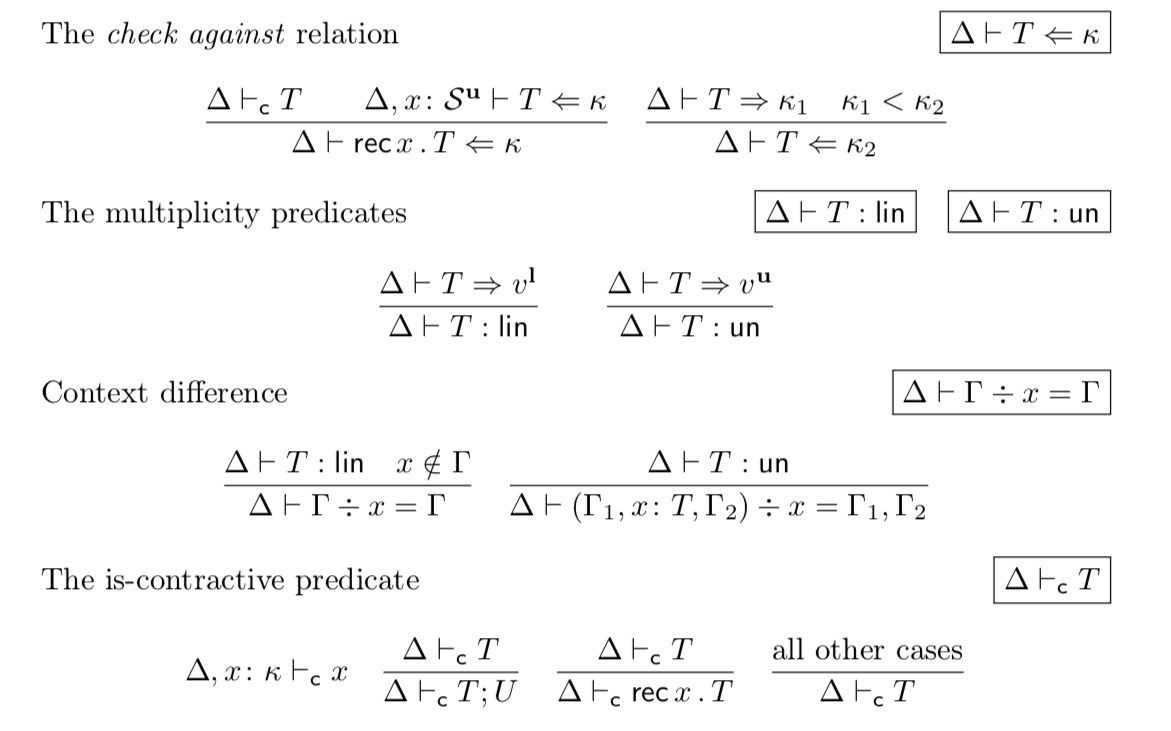
\includegraphics[width=12cm]{img/kinding}	
\end{frame}


}


\end{document}

%%% Local Variables:
%%% mode: latex
%%% TeX-master: t
%%% End:
